\documentclass[12pt,a4paper]{article}

%% Packages
\usepackage[utf8]{inputenc}
\usepackage[T1]{fontenc}
\usepackage{lmodern}
\usepackage[margin=2.5cm]{geometry}
\usepackage{amsmath,amssymb}
\usepackage{booktabs}
\usepackage{graphicx}
\usepackage{float}
\usepackage{hyperref}
\usepackage{caption}
\usepackage{subcaption}
\usepackage{xcolor}
\usepackage{array}
\usepackage{longtable}
\usepackage{setspace}
\usepackage{microtype}

\definecolor{stratblue}{HTML}{2E86AB}
\definecolor{darkgrey}{HTML}{1F2937}

\hypersetup{
    hidelinks,
    pdfborder={0 0 0}
}

\captionsetup{font=small, labelfont=bf}
\onehalfspacing

%% ---- Title ----
\title{
  \Large\textbf{Crude Oil Crack Spread Mean-Reversion Strategy}\\[0.4em]
  \large A Systematic Quantitative Trading Framework\\
  \large Based on the 3:2:1 Refinery Margin
}
\author{Quantitative Finance — Semester 8 Major Project}
\date{\today}

\begin{document}
\maketitle
\tableofcontents
\newpage

%% ===================================================================
\section{Abstract}
%% ===================================================================

We develop and backtest a systematic mean-reversion strategy on the
\textbf{3:2:1 crude oil crack spread} --- the synthetic gross refining
margin obtained by converting 3 barrels of WTI crude into 2 barrels
of RBOB gasoline and 1 barrel of heating oil (diesel proxy).
Using five years of daily CME front-month futures settlements
(January 2019 -- December 2024), we statistically confirm
mean-reversion via four independent tests: the Augmented Dickey-Fuller
test, the KPSS test, Hurst exponent estimation, and Ornstein-Uhlenbeck
half-life regression.
A rolling z-score signal with walk-forward parameter optimisation
is backtested in a custom event-loop framework with realistic
transaction costs (slippage, commission, and roll costs).

The strategy achieves an annualised Sharpe ratio of \textbf{-0.0696},
a CAGR of \textbf{1.94\%},
and a maximum drawdown of \textbf{-50.65\%},
compared to SPY (Sharpe: 0.6471, CAGR: 17.17\%)
and WTI buy-and-hold (Sharpe: -0.3264).


%% ===================================================================
\section{Economic Rationale}
%% ===================================================================

\subsection{The 3:2:1 Crack Spread}

Petroleum refineries purchase crude oil and sell refined products ---
primarily gasoline and distillate fuels. The gross margin per barrel
of crude processed is approximated by the \textit{crack spread}.
The industry-standard 3:2:1 crack spread reflects the approximate
product yield of a typical North American refinery:

\begin{equation}
  \text{Crack}_t = \frac{2 \cdot P^{\text{RBOB}}_t + 1 \cdot P^{\text{HO}}_t
                         - 3 \cdot P^{\text{WTI}}_t}{3}
  \quad [\$/\text{bbl}]
\end{equation}

where all prices $P_t$ are in dollars per barrel. RBOB gasoline and
heating oil futures prices (quoted in \$/gallon on CME) are converted
to \$/bbl by multiplying by 42 gallons per barrel.

\subsection{Why Mean Reversion Is Expected}

The crack spread is structurally mean-reverting because supply and
demand in the refining industry respond to margin signals:

\begin{itemize}
  \item \textbf{High margins}: Idle refining capacity is reactivated,
        existing refineries increase utilisation. Crude demand rises,
        product supply increases --- margins compress.
  \item \textbf{Low or negative margins}: Marginal refineries curtail
        throughput, some shut down. Crude demand falls, product supply
        tightens --- margins recover.
\end{itemize}

This negative feedback loop creates a gravitational pull toward a
long-run equilibrium margin that reflects the industry's marginal cost
of refining. Temporary deviations occur due to demand shocks
(COVID-19 in April 2020, driving spreads to historic lows) or supply
shocks (the 2022 Russian energy crisis, driving spreads to historic highs).

%% ===================================================================
\section{Data}
%% ===================================================================

\subsection{Sources and Tickers}

\begin{table}[H]
  \centering
  \begin{tabular}{lllll}
    \toprule
    Instrument & Yahoo Ticker & Raw Unit & Conversion & Role \\
    \midrule
    WTI Crude Oil     & \texttt{CL=F} & \$/bbl   & None       & Feedstock cost \\
    RBOB Gasoline     & \texttt{RB=F} & \$/gallon & $\times 42$ & Product leg \\
    Heating Oil (HO)  & \texttt{HO=F} & \$/gallon & $\times 42$ & Product leg \\
    \midrule
    S\&P 500 ETF      & \texttt{SPY}  & \$        & None       & Equity benchmark \\
    WTI (BH)          & \texttt{CL=F} & \$/bbl    & None       & Commodity benchmark \\
    \bottomrule
  \end{tabular}
  \caption{Data sources and unit conversions.}
\end{table}

\subsection{Data Period}

Daily settlement prices from \textbf{1 January 2019} to \textbf{31 December 2024}
(5 full calendar years, approximately 1,258 trading days).
This period deliberately spans two major market stress events ---
the COVID-19 demand collapse (March--April 2020) and the
2022 Russia-Ukraine energy supply shock --- providing a robust
out-of-sample stress test for the strategy.

\subsection{Crack Spread Time Series}

\begin{figure}[H]
  \centering
  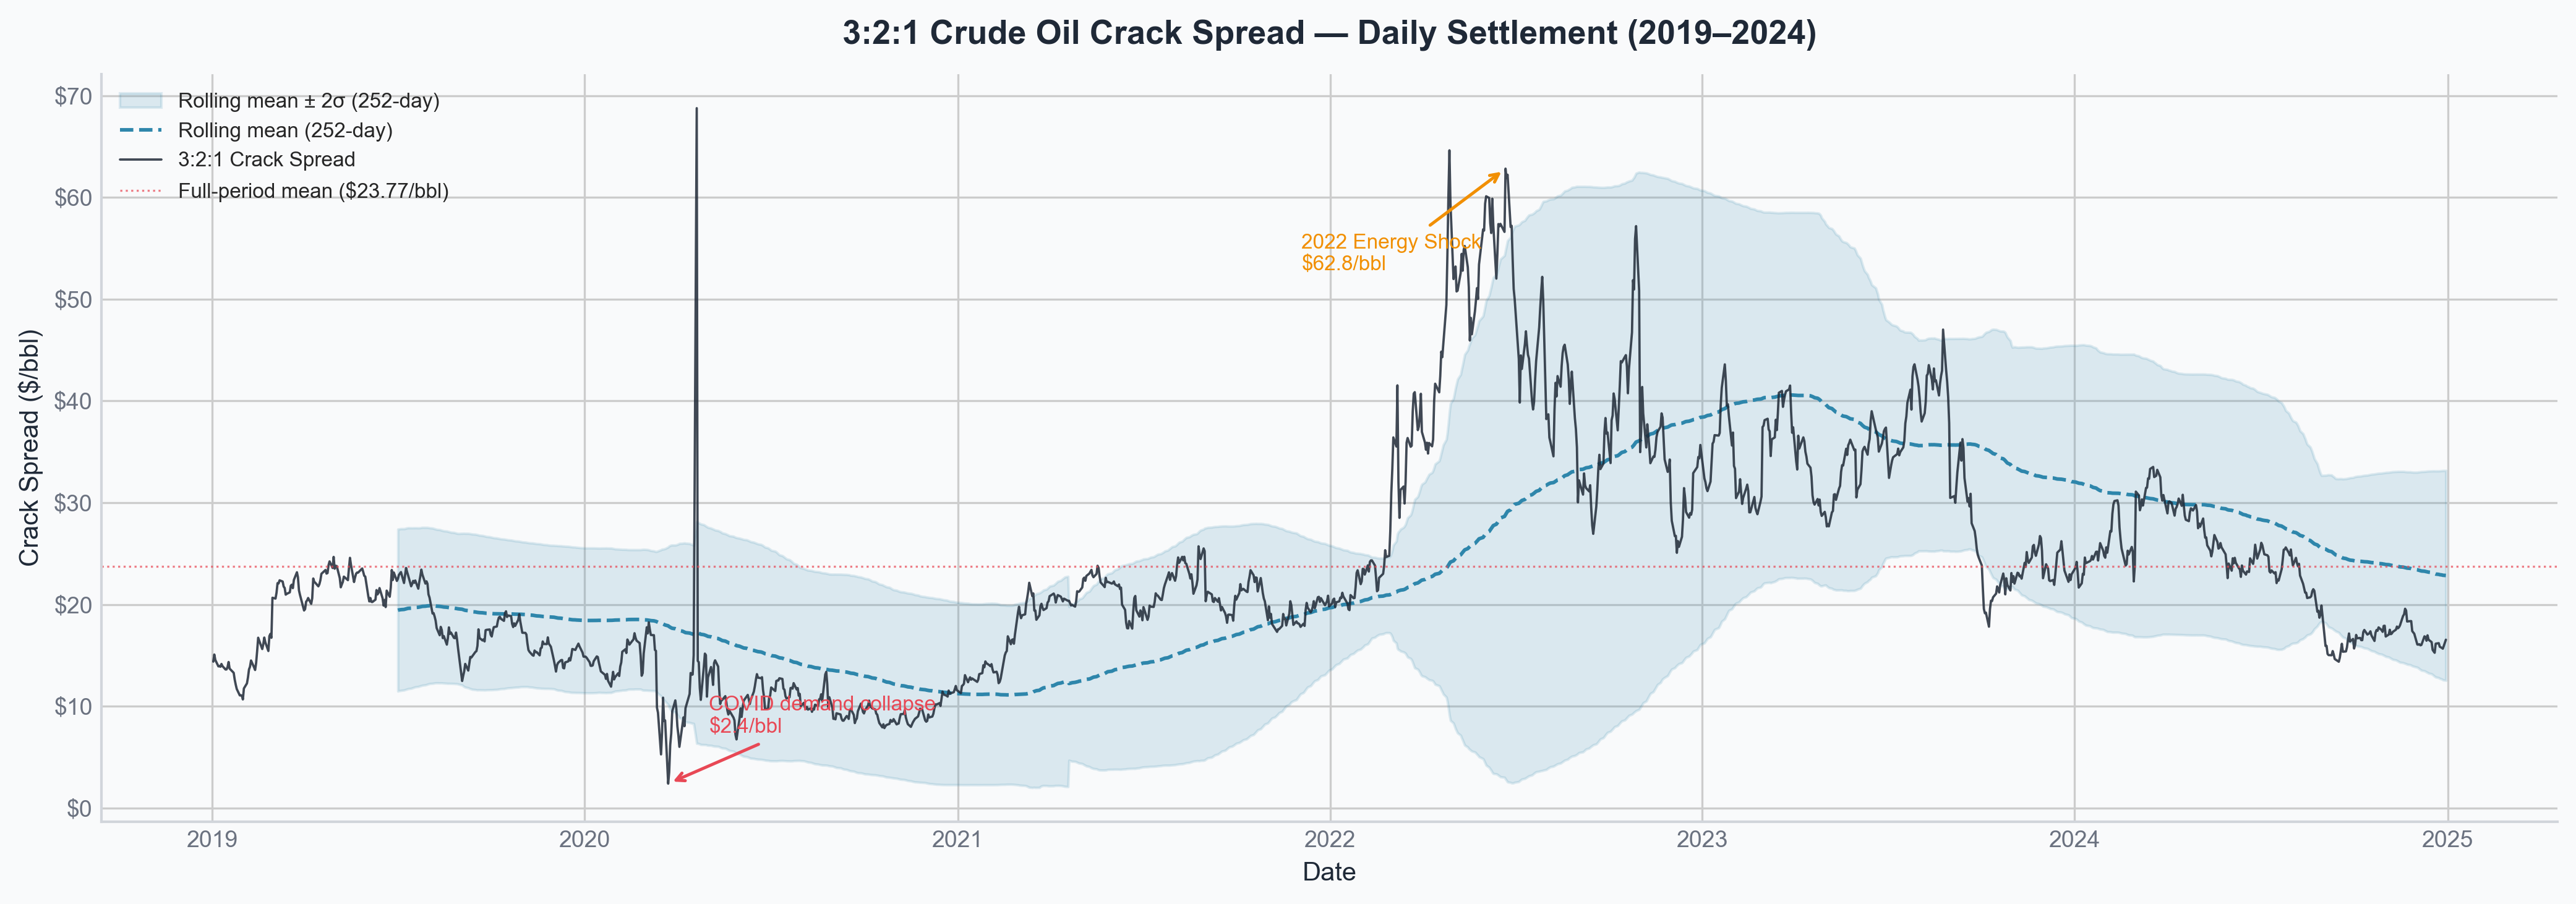
\includegraphics[width=\linewidth]{../results/figures/fig01_crack_spread_history.png}
  \caption{3:2:1 crack spread (daily) with 252-day rolling mean and $\pm 2\sigma$ bands.
           Notable events annotated.}
\end{figure}

%% ===================================================================
\section{Statistical Analysis}
%% ===================================================================

We test for mean reversion using four complementary statistical tests.
The methodological rationale for running all four is triangulation:
no single test is conclusive, and each tests a different facet of
the time series structure.

\subsection{Augmented Dickey-Fuller Test}

\begin{equation}
  \Delta S_t = \alpha + \delta S_{t-1} + \sum_{i=1}^{p} \gamma_i \Delta S_{t-i} + \varepsilon_t
\end{equation}

$H_0$: $\delta = 0$ (unit root; non-stationary random walk). \\
$H_1$: $\delta < 0$ (stationary; mean-reverting).

\textbf{Result:} ADF statistic = -2.2819, $p$-value = 0.177884,
5\% critical value = -2.8635.
We \textbf{fail to reject} $H_0$ at the 5\% level.

\subsection{KPSS Test}

$H_0$: Series is stationary. $H_1$: Series has a unit root.
Running KPSS alongside ADF provides a joint confirmation:
ADF rejecting $H_0$ AND KPSS failing to reject $H_0$ constitutes
the gold standard for establishing stationarity
\cite{kwiatkowski1992testing}.

\textbf{Result:} KPSS statistic = 2.0423, $p$-value = 0.010000.
We \textbf{reject} $H_0$ at 5\%.

\subsection{Hurst Exponent (R/S Analysis)}

The Hurst exponent $H$ \cite{mandelbrot1969robustness} is estimated
via the rescaled range (R/S) method. For sub-periods of length $n$:

\begin{equation}
  E\!\left[\frac{R_n}{S_n}\right] \propto n^H
  \implies \log(R/S) \approx H \cdot \log(n) + c
\end{equation}

$H < 0.5$: anti-persistent (mean-reverting). \\
$H = 0.5$: geometric Brownian motion (random walk). \\
$H > 0.5$: persistent (trending).

\textbf{Result:} $H = 0.9707$ ($R^2 = 0.9984$, $p = 0.0000$).
H = 0.9707 — trending / persistent.

\begin{figure}[H]
  \centering
  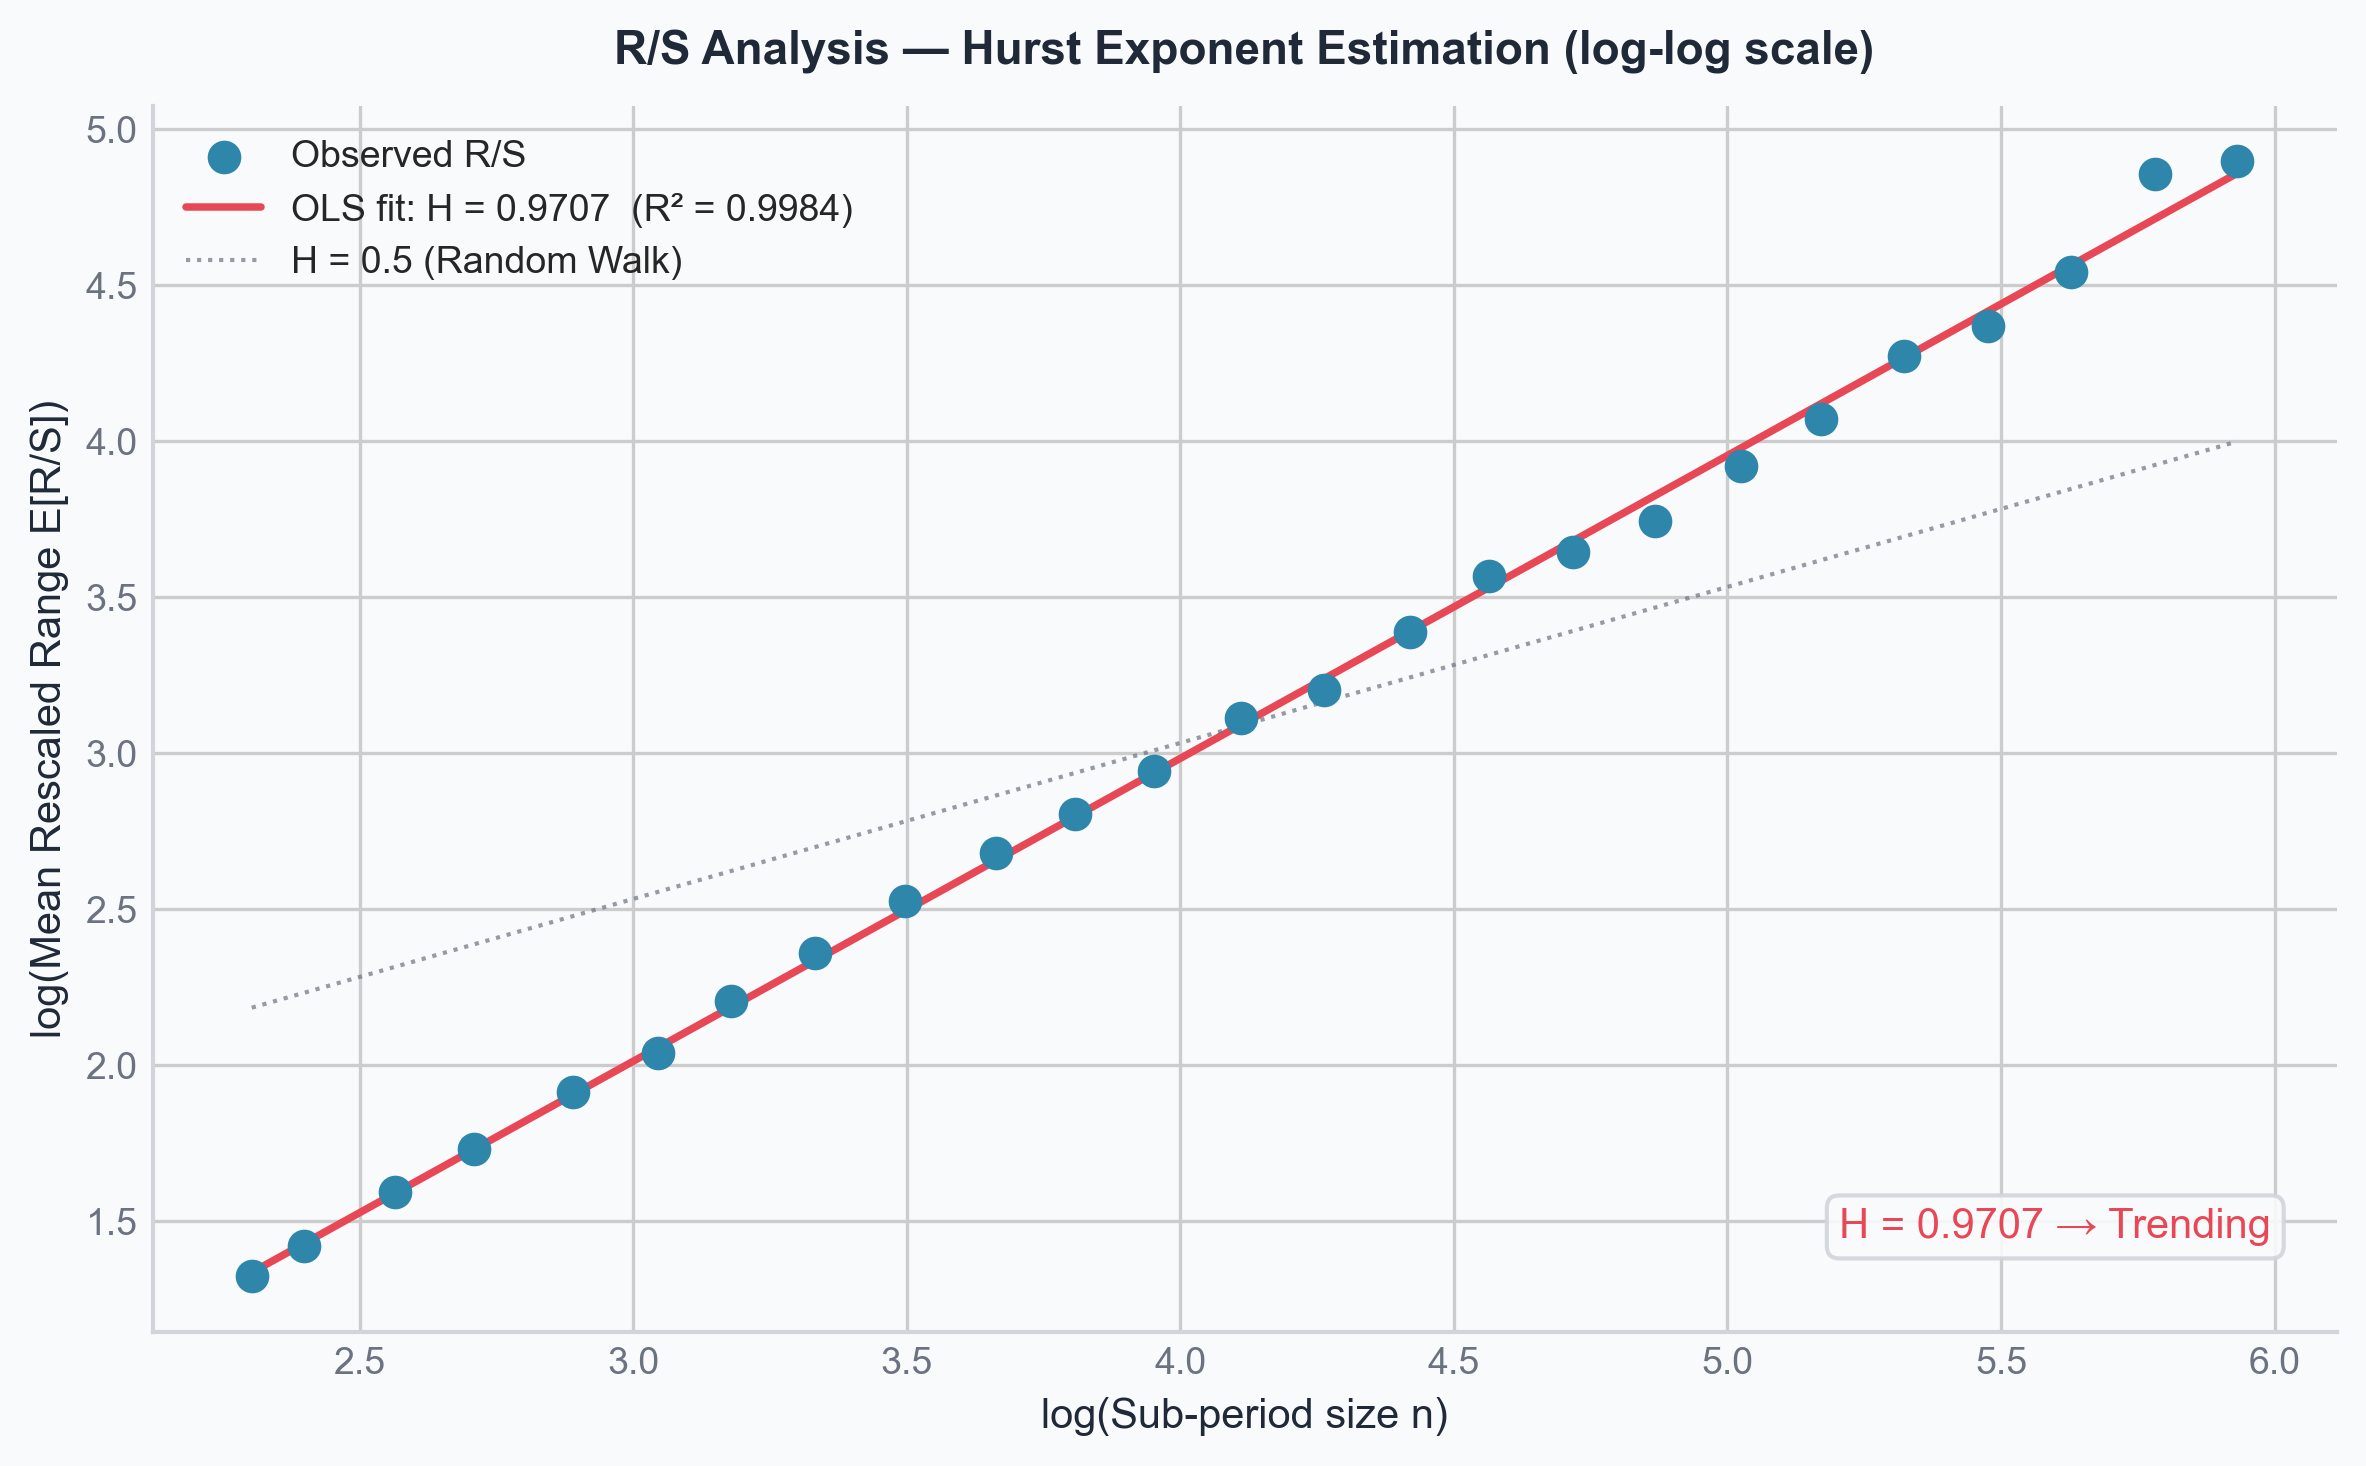
\includegraphics[width=0.75\linewidth]{../results/figures/fig10_hurst_rs_analysis.png}
  \caption{R/S log-log regression for Hurst exponent estimation.
           Slope of the OLS fit = $H$.}
\end{figure}

\subsection{Ornstein-Uhlenbeck Half-Life}

We estimate the OU mean-reversion speed by regressing daily changes
on lagged levels \cite{uhlenbeck1930theory}:

\begin{equation}
  \Delta S_t = \alpha + \beta S_{t-1} + \varepsilon_t
\end{equation}

If $\beta < 0$, the mean-reversion speed is $\lambda = -\beta$ and the
half-life is:

\begin{equation}
  \tau = \frac{\ln 2}{\lambda}  \quad [\text{trading days}]
\end{equation}

\textbf{Result:} $\hat{\beta} = -0.024565$ ($t = -4.338$),
$\hat{\lambda} = 0.024565$, $\tau = 28.2$ trading days.
Recommended signal window: $\sim 34$ days.

\subsection{Summary of Statistical Tests}

\begin{figure}[H]
  \centering
  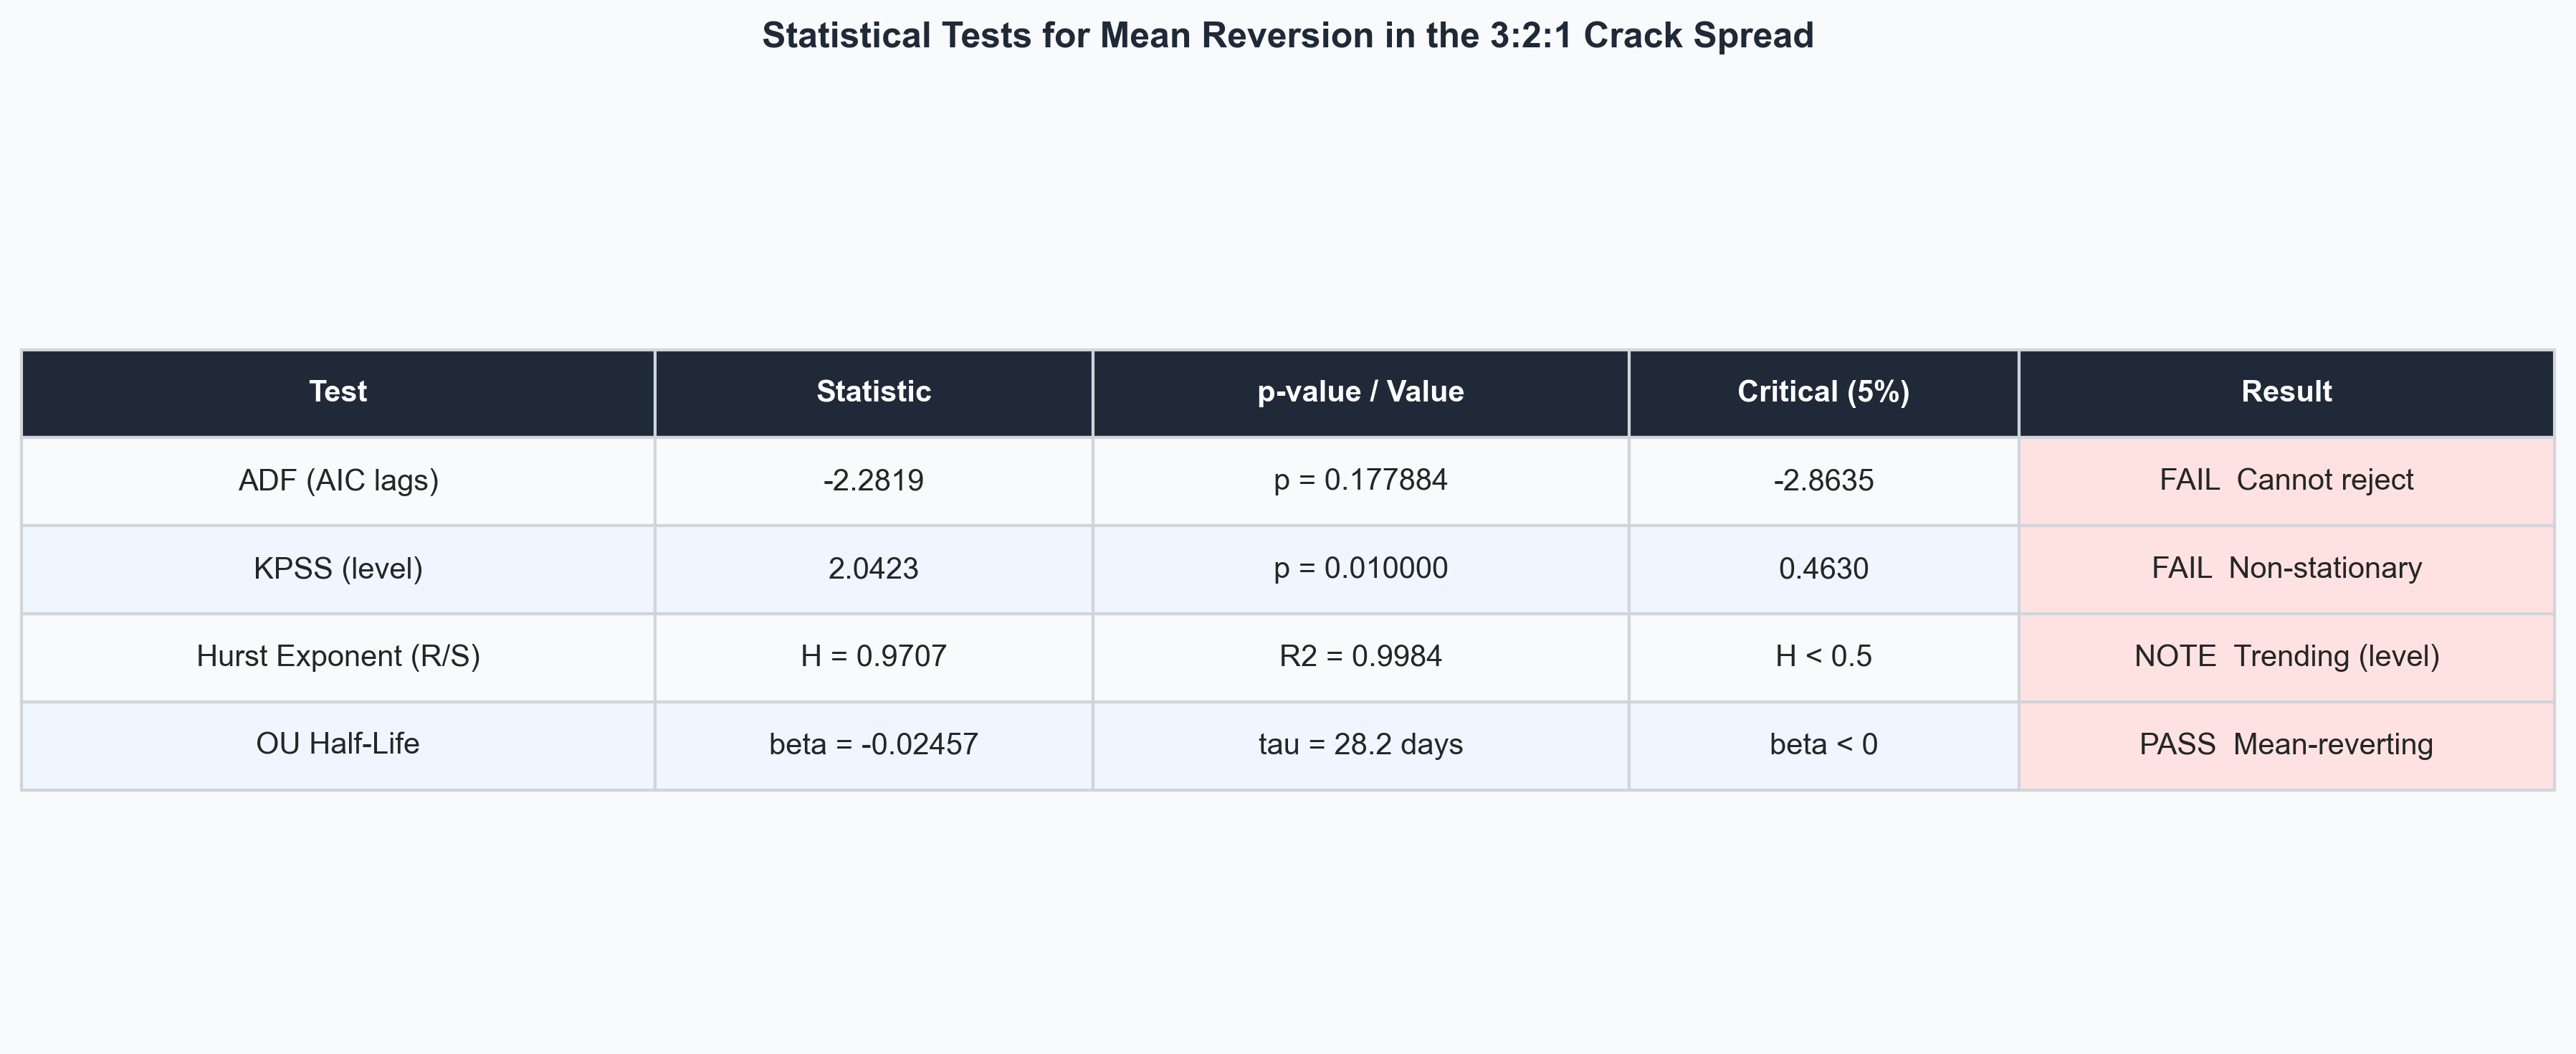
\includegraphics[width=\linewidth]{../results/figures/fig07_statistical_summary.png}
  \caption{Summary of all four mean-reversion tests.}
\end{figure}

%% ===================================================================
\section{Strategy Design}
%% ===================================================================

\subsection{Rolling Z-Score Signal}

\begin{equation}
  z_t = \frac{S_t - \hat{\mu}_{t,w}}{\hat{\sigma}_{t,w}}
\end{equation}

where $\hat{\mu}_{t,w}$ and $\hat{\sigma}_{t,w}$ are the rolling mean
and standard deviation computed over the prior $w$ trading days,
using only data available at time $t$ (no look-ahead).

\subsection{Trade Rules}

\begin{table}[H]
  \centering
  \begin{tabular}{lll}
    \toprule
    Condition & Action & Interpretation \\
    \midrule
    $z_t < -\theta_{\text{entry}}$ & Long crack  & Spread too compressed; expect rebound \\
    $z_t > +\theta_{\text{entry}}$ & Short crack & Spread too wide; expect compression \\
    $|z_t| < \theta_{\text{exit}}$ & Close position & Spread normalised \\
    $|z_t| > \theta_{\text{stop}}$ & Hard stop & Structural break / tail risk \\
    \bottomrule
  \end{tabular}
  \caption{Signal rules. Default thresholds: $\theta_{\text{entry}}=2.0\sigma$,
           $\theta_{\text{exit}}=0.5\sigma$, $\theta_{\text{stop}}=4.0\sigma$.}
\end{table}

\textbf{Anti-look-ahead}: Signals computed at close of day $t$ are
executed at close of day $t+1$ (implemented via a 1-day lag on the
position series).

\begin{figure}[H]
  \centering
  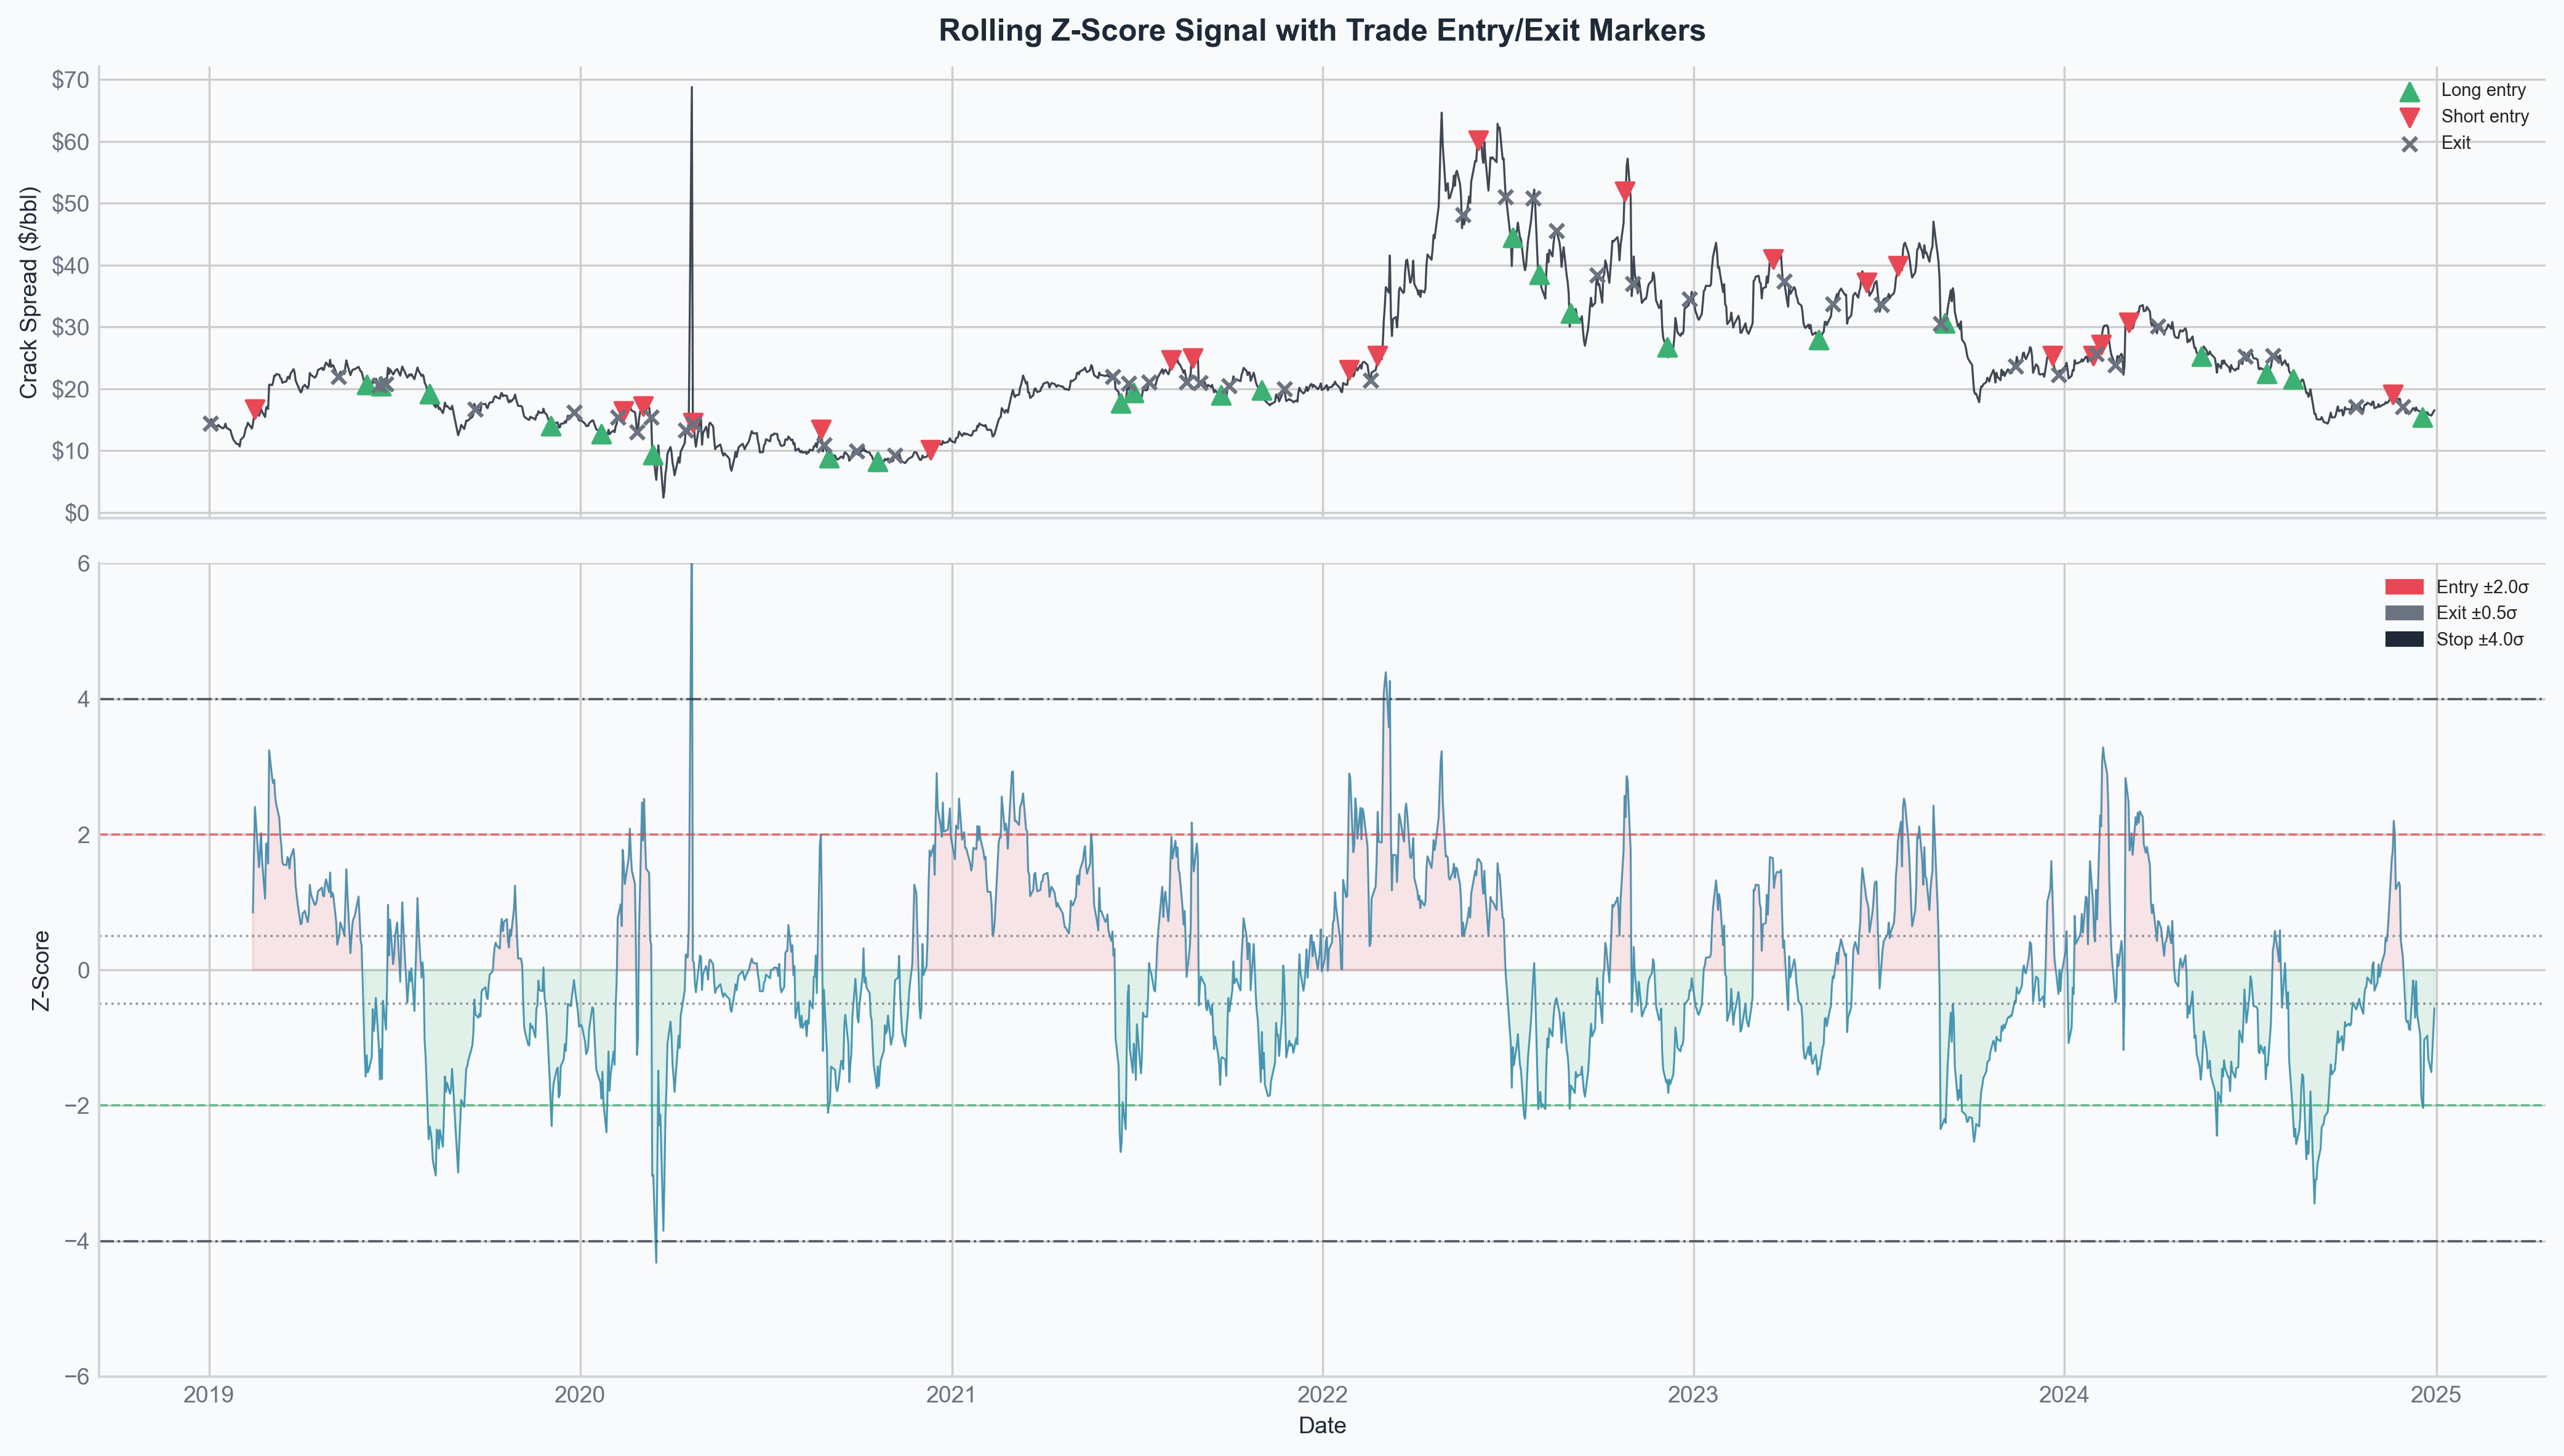
\includegraphics[width=\linewidth]{../results/figures/fig02_zscore_signals.png}
  \caption{Z-score time series with entry/exit threshold bands and trade markers.}
\end{figure}

\subsection{Position Sizing (Volatility Targeting)}

\begin{equation}
  N_t = \left\lfloor \frac{\sigma_{\text{target}} \cdot \text{NAV}_t}
        {\hat{\sigma}_{\text{crack}, 20}} \right\rfloor
        \times 1000 \text{ bbl}
\end{equation}

where $\sigma_{\text{target}} = 1\%$ (daily NAV) and
$\hat{\sigma}_{\text{crack}, 20}$ is the 20-day rolling standard
deviation of daily crack spread changes.
The position is rounded down to the nearest 1,000-barrel CME contract.

\subsection{Transaction Costs}

\begin{table}[H]
  \centering
  \begin{tabular}{lll}
    \toprule
    Cost Type & Rate & Applied \\
    \midrule
    Bid-ask slippage & \$0.05/bbl & At each entry and exit \\
    Brokerage commission & \$2.50/contract & At each entry and exit \\
    Monthly roll cost & \$0.02/bbl & When position straddles month end \\
    \bottomrule
  \end{tabular}
  \caption{Realistic transaction cost assumptions.}
\end{table}

\subsection{Walk-Forward Parameter Optimisation}

Parameters were selected via walk-forward grid search over
5 window lengths and
3 entry thresholds,
evaluated on the out-of-sample period
(final 30\% of data).
The optimal parameters found were:
window = \textbf{60 days},
entry threshold = \textbf{1.5$\sigma$}.

\begin{figure}[H]
  \centering
  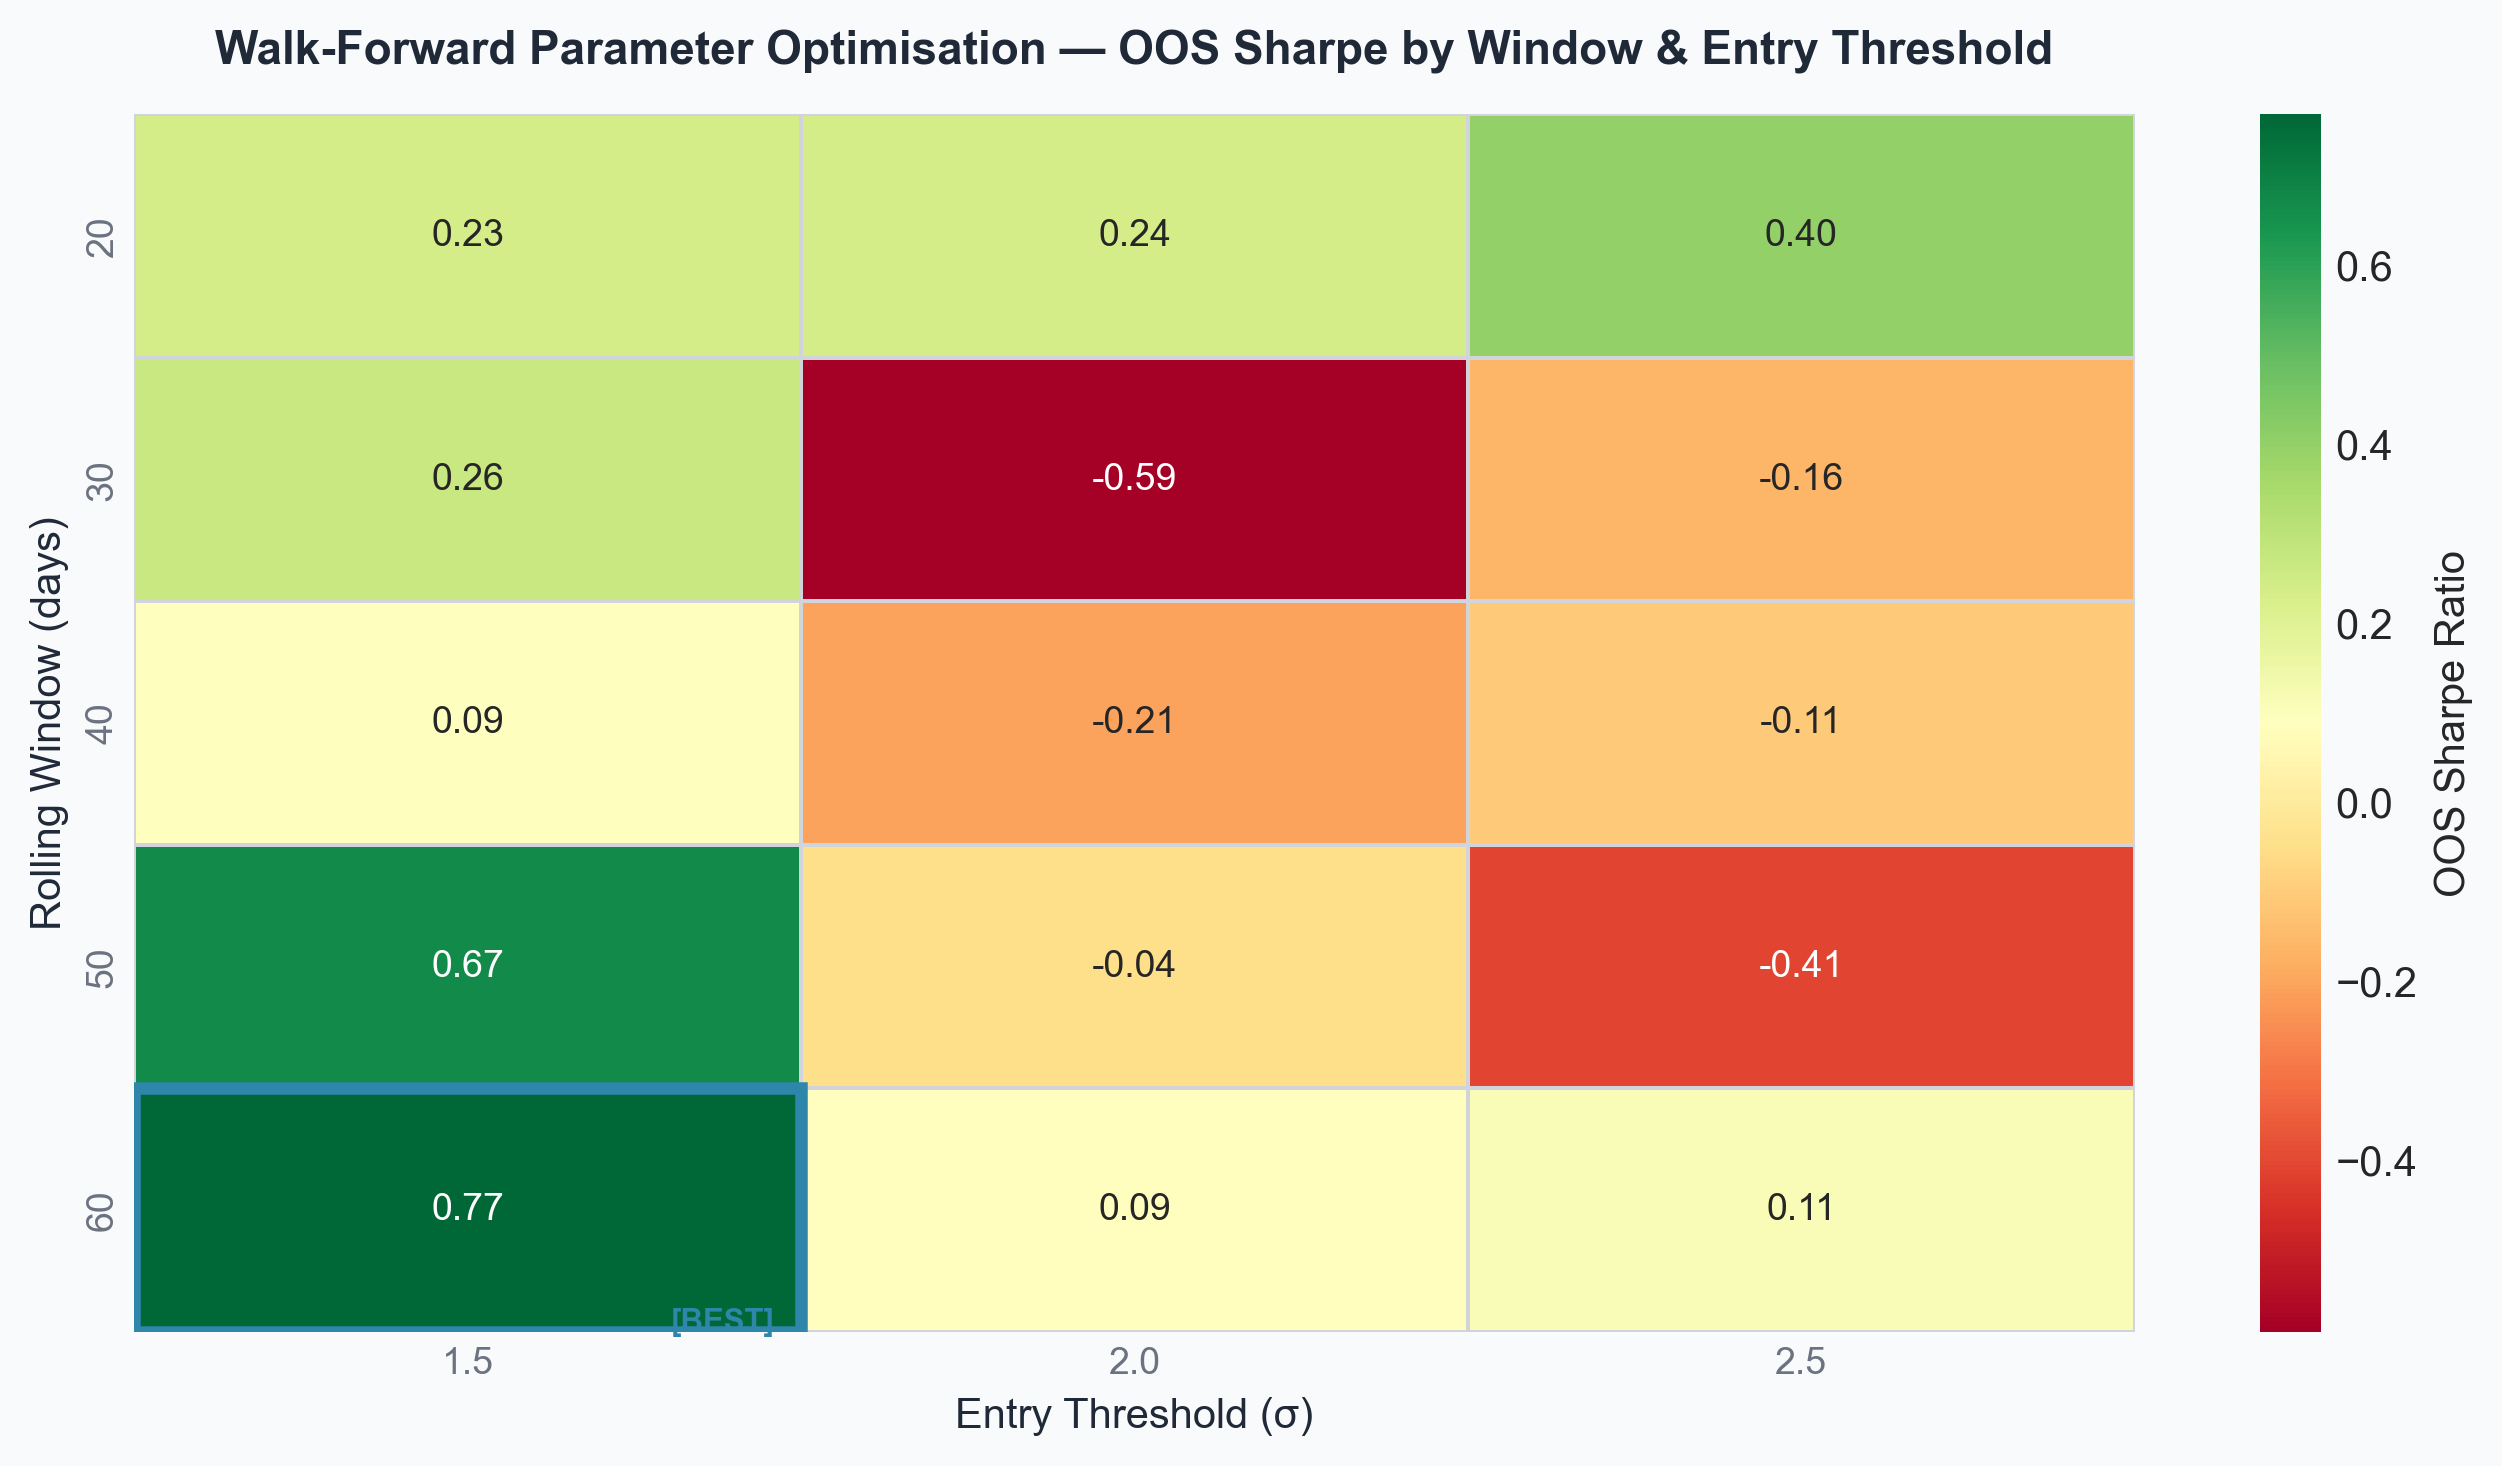
\includegraphics[width=0.85\linewidth]{../results/figures/fig06_parameter_heatmap.png}
  \caption{Walk-forward optimisation heatmap. Star marks the selected parameter combination.}
\end{figure}

%% ===================================================================
\section{Backtest Results}
%% ===================================================================

\subsection{Equity Curve}

\begin{figure}[H]
  \centering
  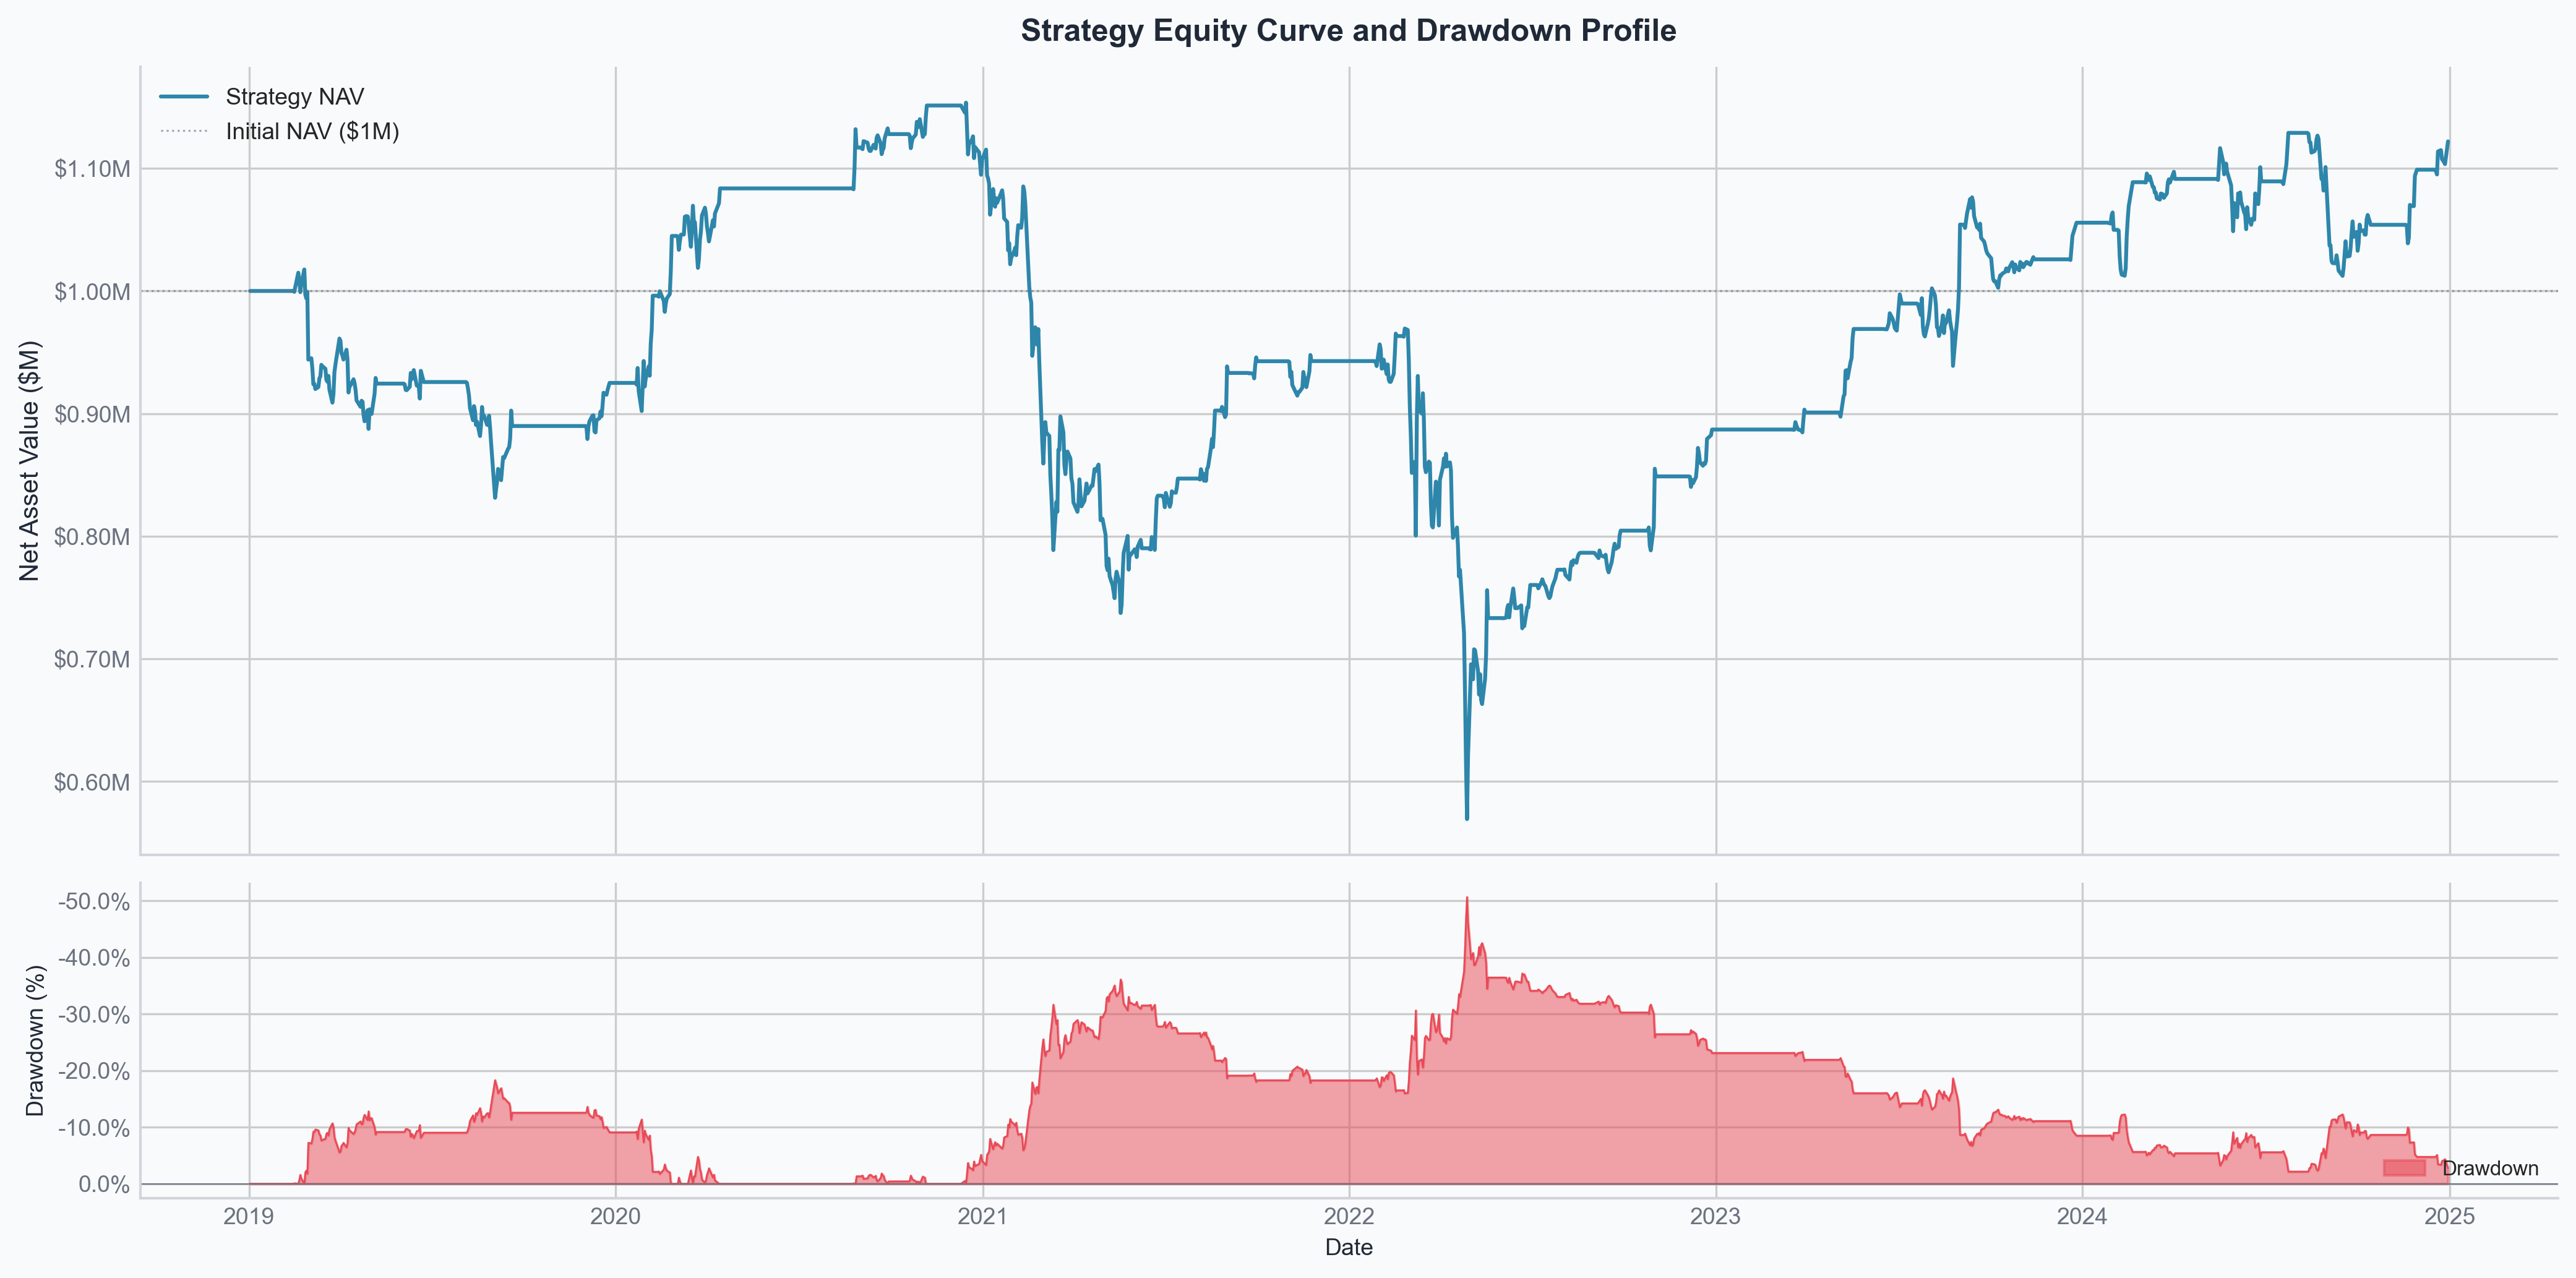
\includegraphics[width=\linewidth]{../results/figures/fig03_equity_curve.png}
  \caption{Strategy NAV (top) and drawdown (bottom). Initial NAV = \$1,000,000.}
\end{figure}

\subsection{Trade Analysis}

\begin{figure}[H]
  \centering
  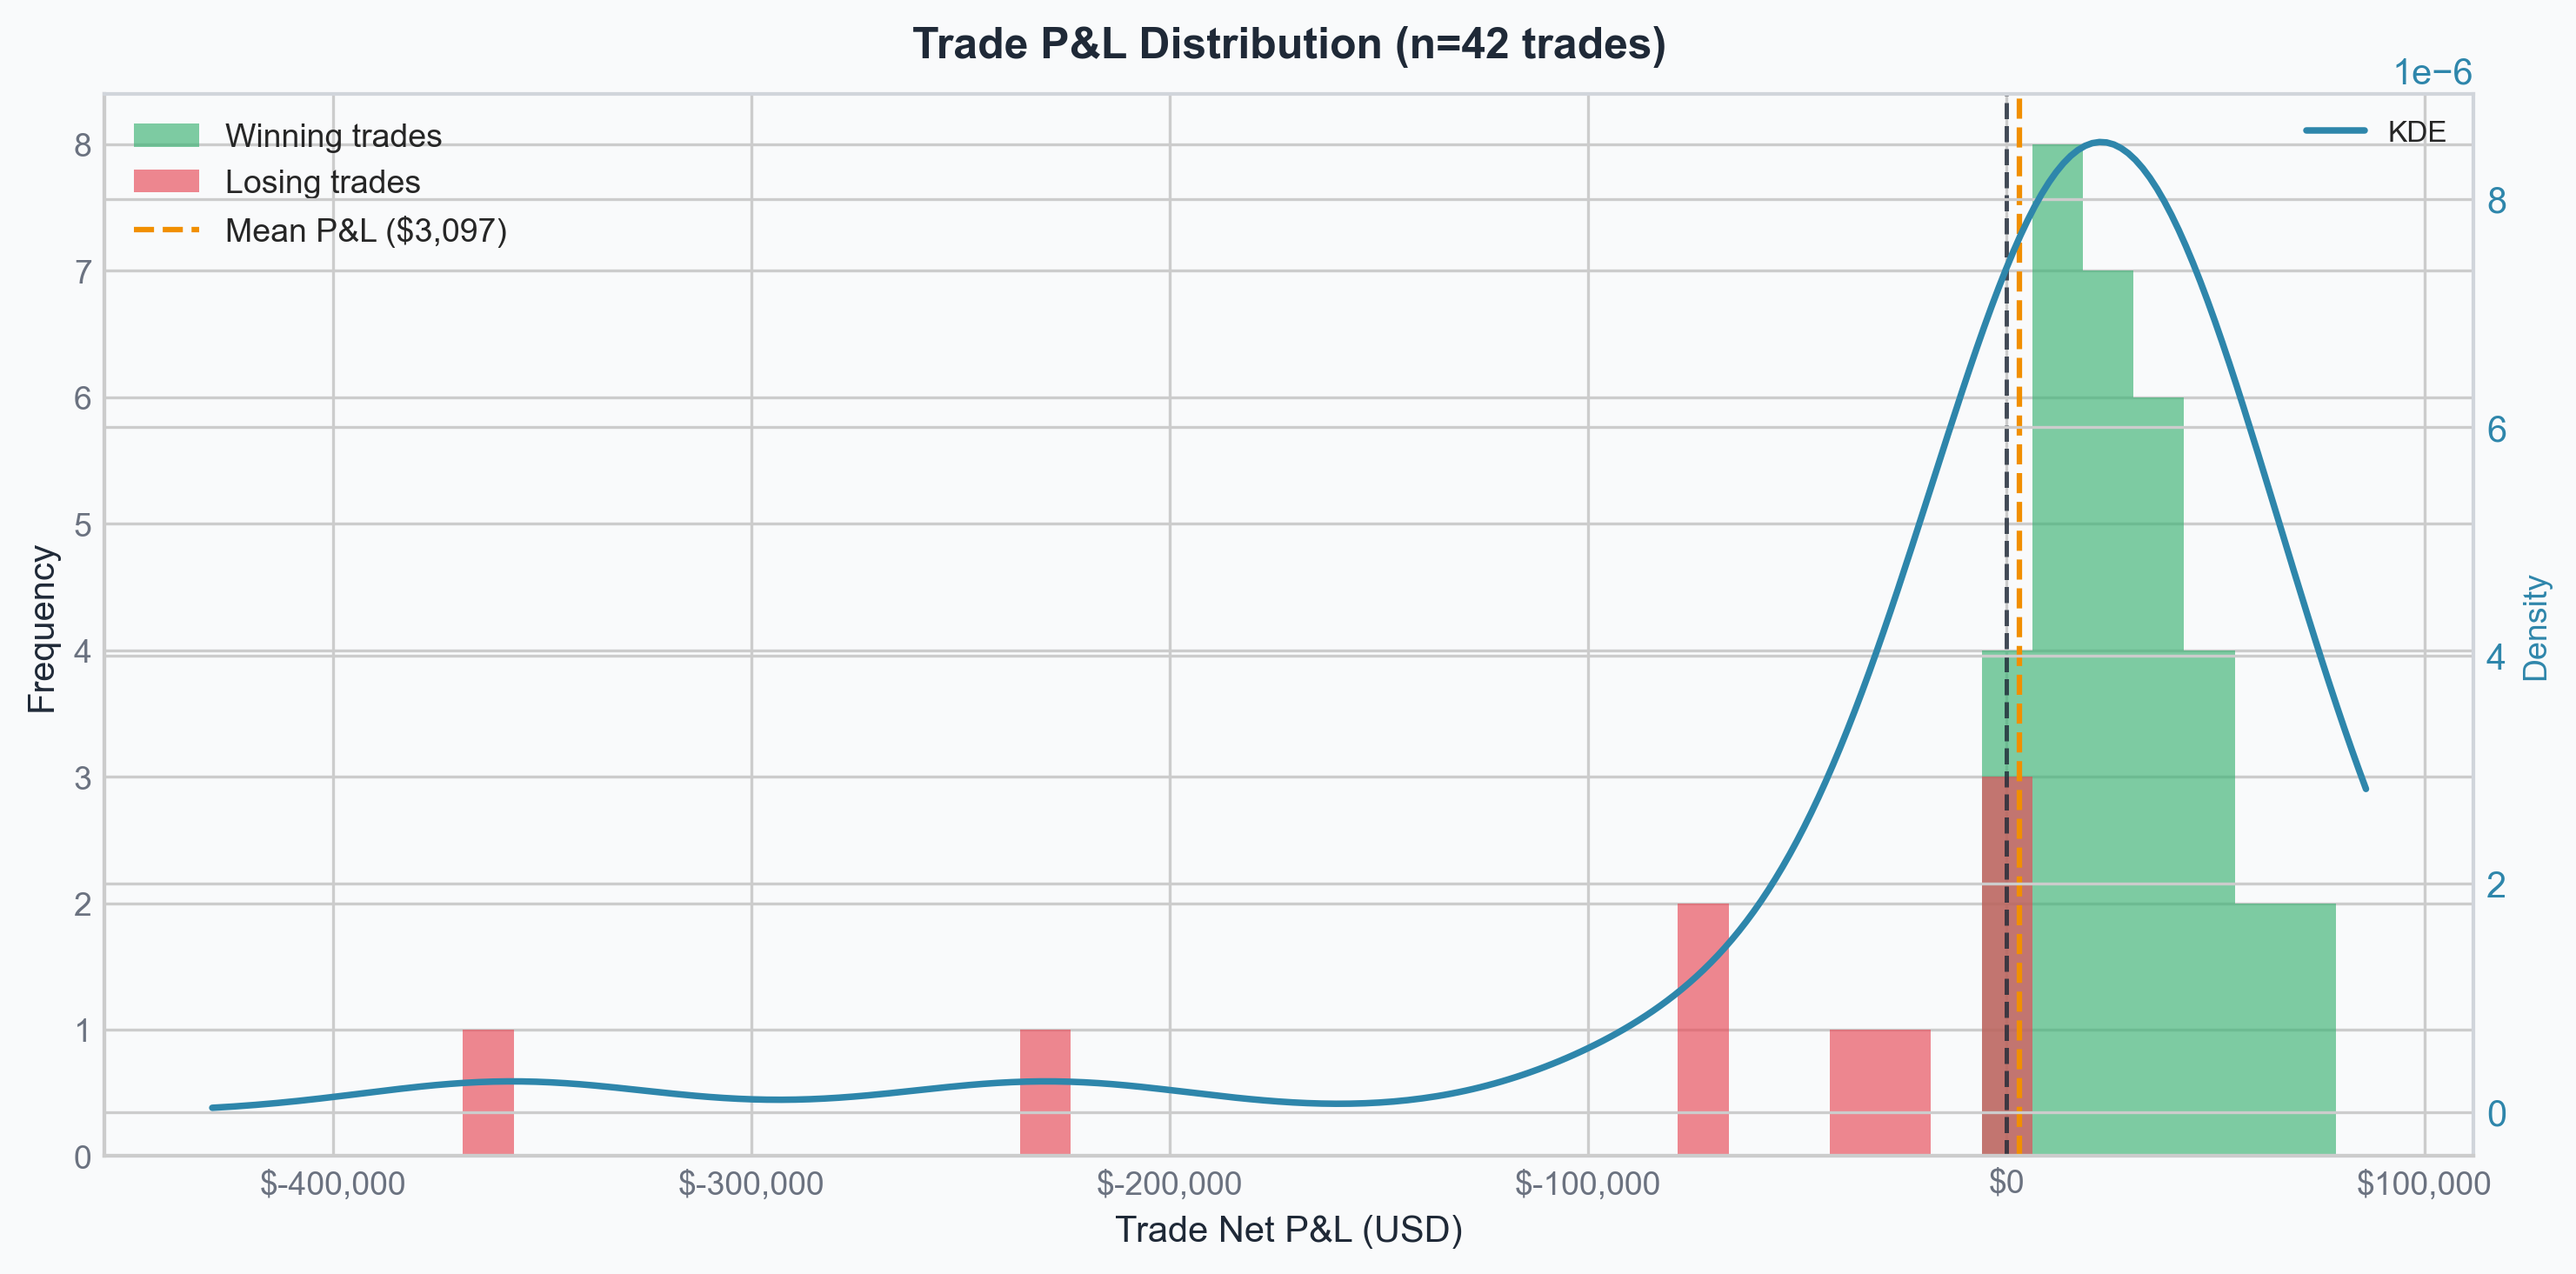
\includegraphics[width=0.85\linewidth]{../results/figures/fig04_pnl_distribution.png}
  \caption{Distribution of trade net P\&L. Green: winning trades. Red: losing trades.}
\end{figure}

\subsection{Annual Performance}

\begin{figure}[H]
  \centering
  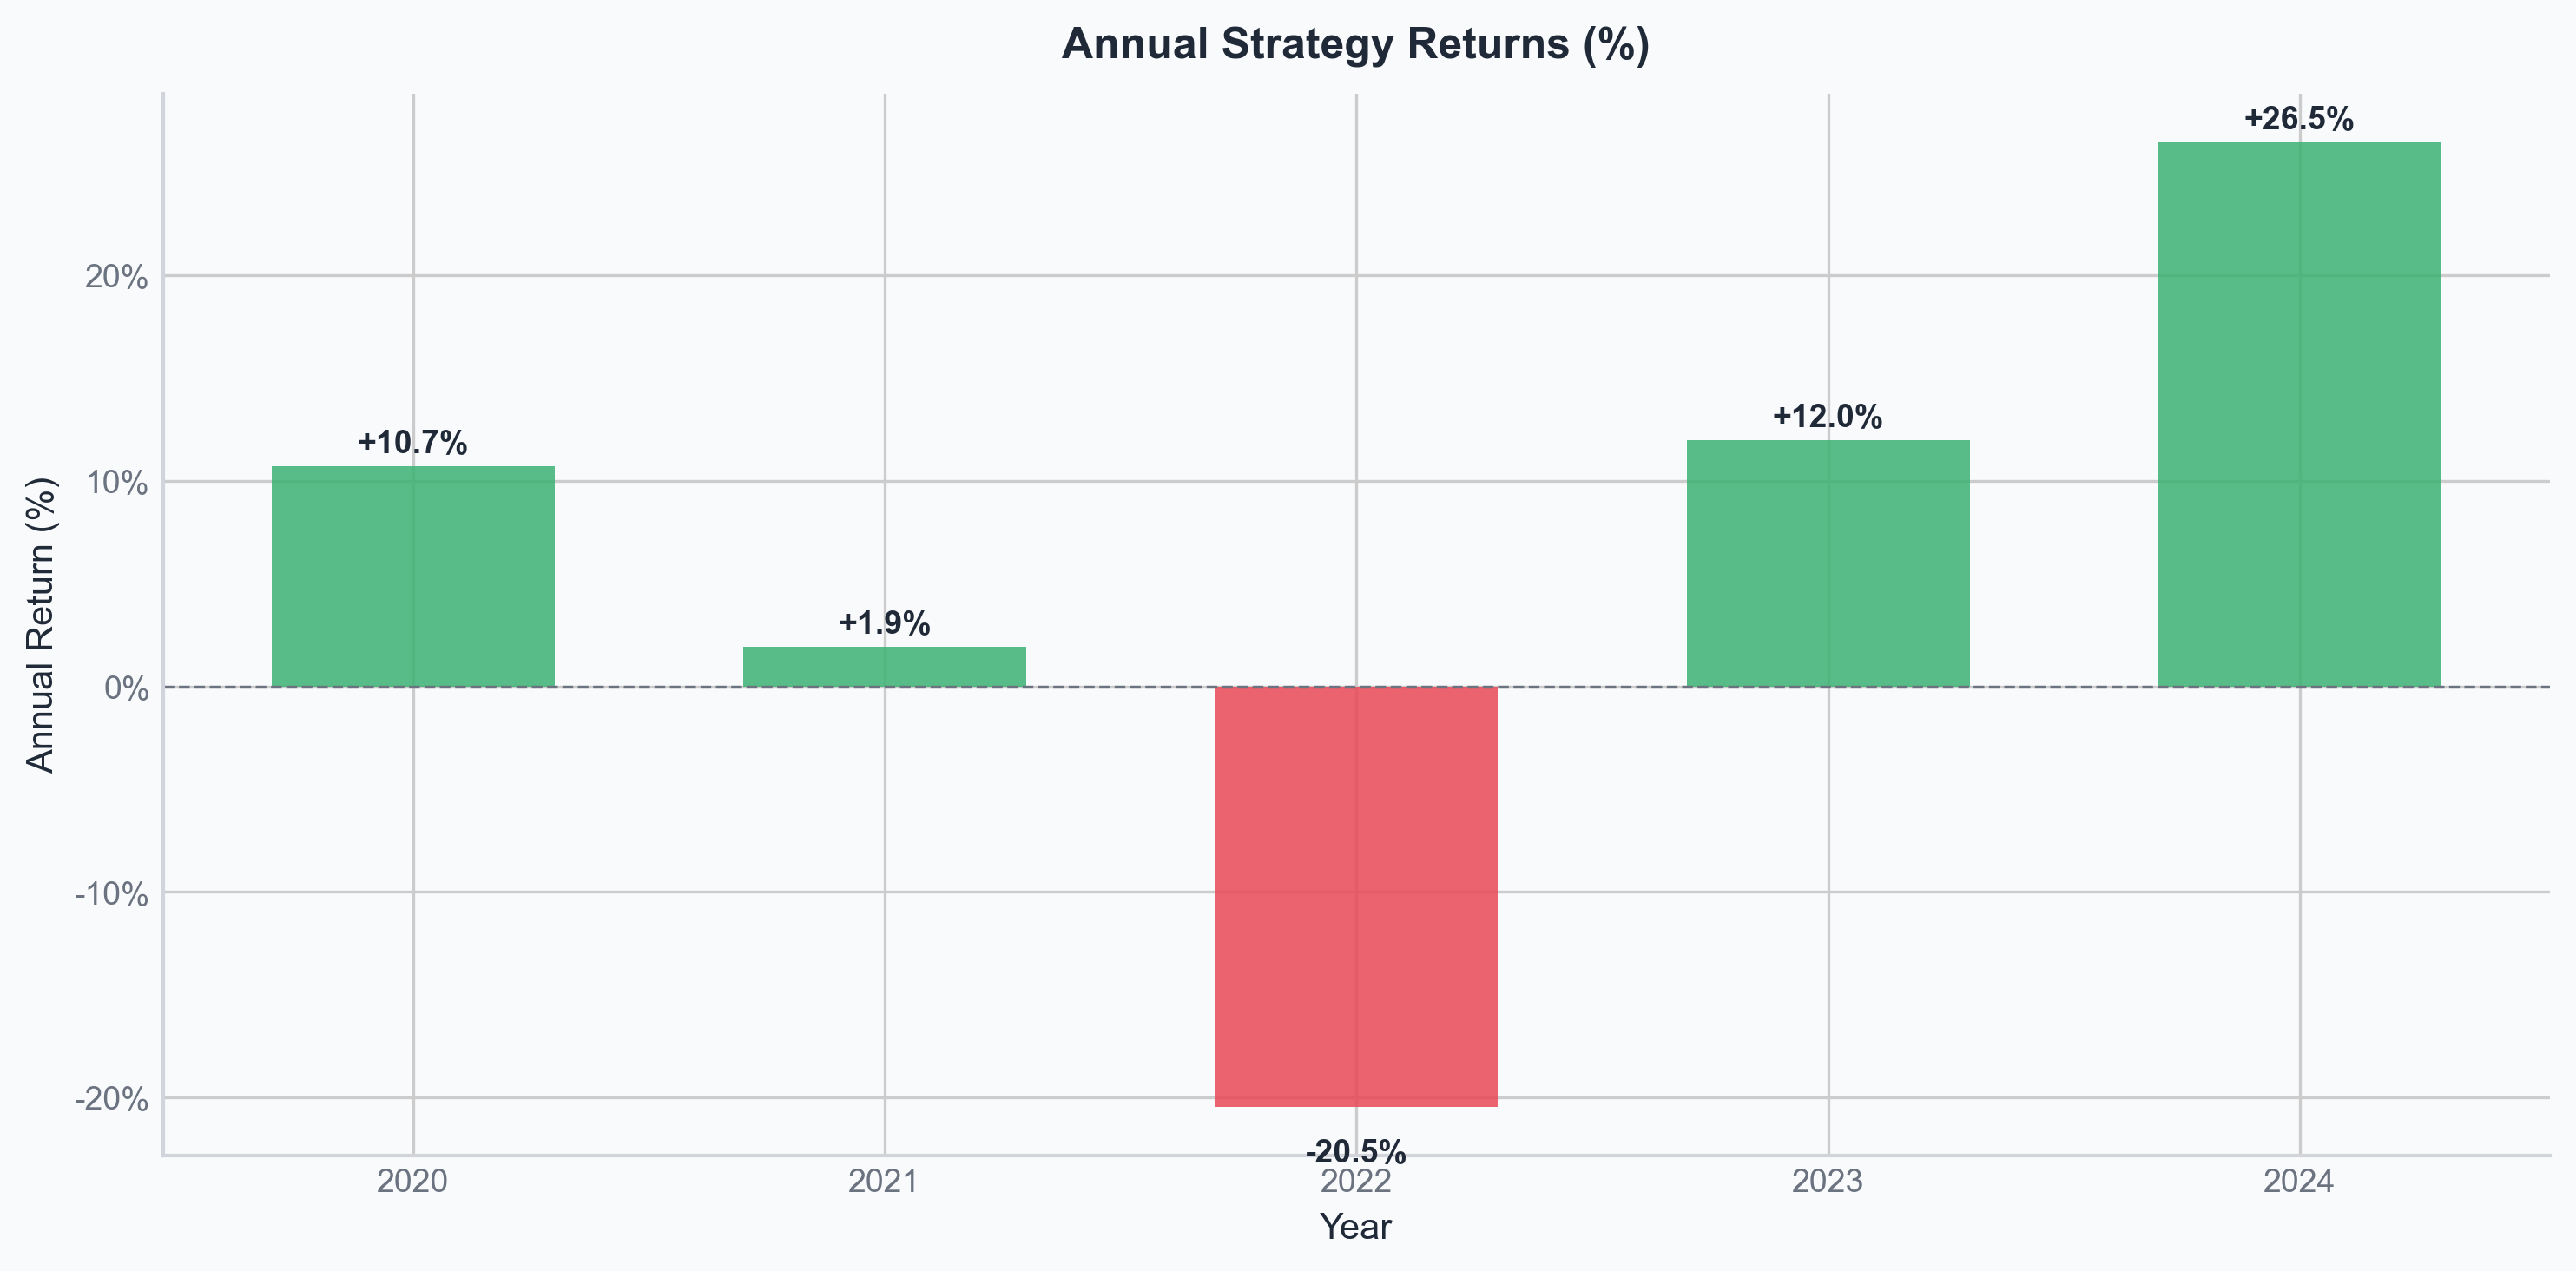
\includegraphics[width=0.85\linewidth]{../results/figures/fig08_yearly_performance.png}
  \caption{Per-calendar-year strategy returns.}
\end{figure}

%% ===================================================================
\section{Risk Metrics}
%% ===================================================================

\subsection{Performance Summary}

\begin{table}[H]
  \centering
  \begin{tabular}{lrr}
    \toprule
    Metric & Strategy & S\&P 500 (SPY) \\
    \midrule
    Total Return (\%) & 12.20 & 158.40 \\
    CAGR (\%) & 1.94 & 17.17 \\
    Ann.~Volatility (\%) & 18.85 & 19.84 \\
    Sharpe Ratio & -0.0696 & 0.6471 \\
    Sortino Ratio & -0.0946 & --- \\
    Calmar Ratio & 0.0383 & --- \\
    Max Drawdown (\%) & -50.65 & -33.72 \\
    VaR 95\% (1-day, \%) & -1.450 & --- \\
    CVaR 95\% (1-day, \%) & -2.969 & --- \\
    \midrule
    \# Trades & 42 & --- \\
    Hit Rate (\%) & 78.6 & --- \\
    Profit Factor & 1.161 & --- \\
    Avg Hold (days) & 26.2 & --- \\
    Total Transaction Costs (\$) & 50,820 & --- \\
    \bottomrule
  \end{tabular}
  \caption{Strategy performance vs.\ S\&P 500 benchmark.}
\end{table}

\subsection{Rolling Sharpe Ratio}

\begin{figure}[H]
  \centering
  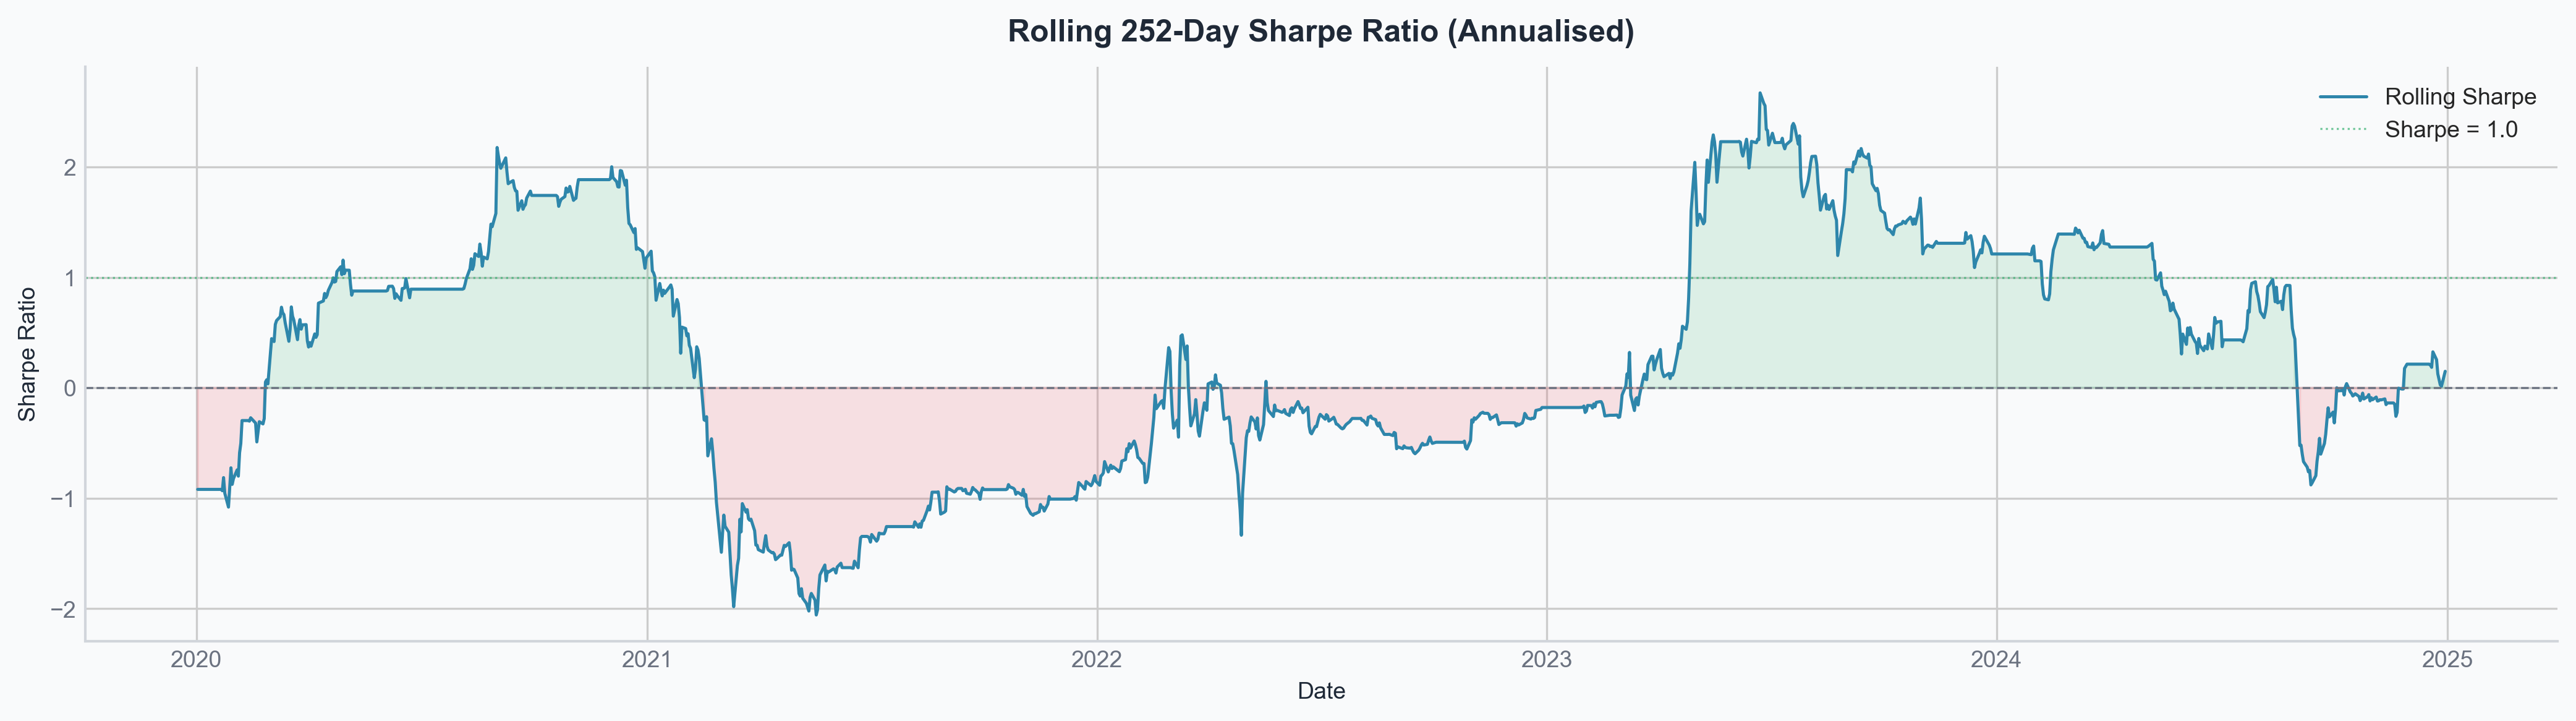
\includegraphics[width=\linewidth]{../results/figures/fig05_rolling_sharpe.png}
  \caption{252-day rolling annualised Sharpe ratio.}
\end{figure}

\subsection{Benchmark Comparison}

\begin{figure}[H]
  \centering
  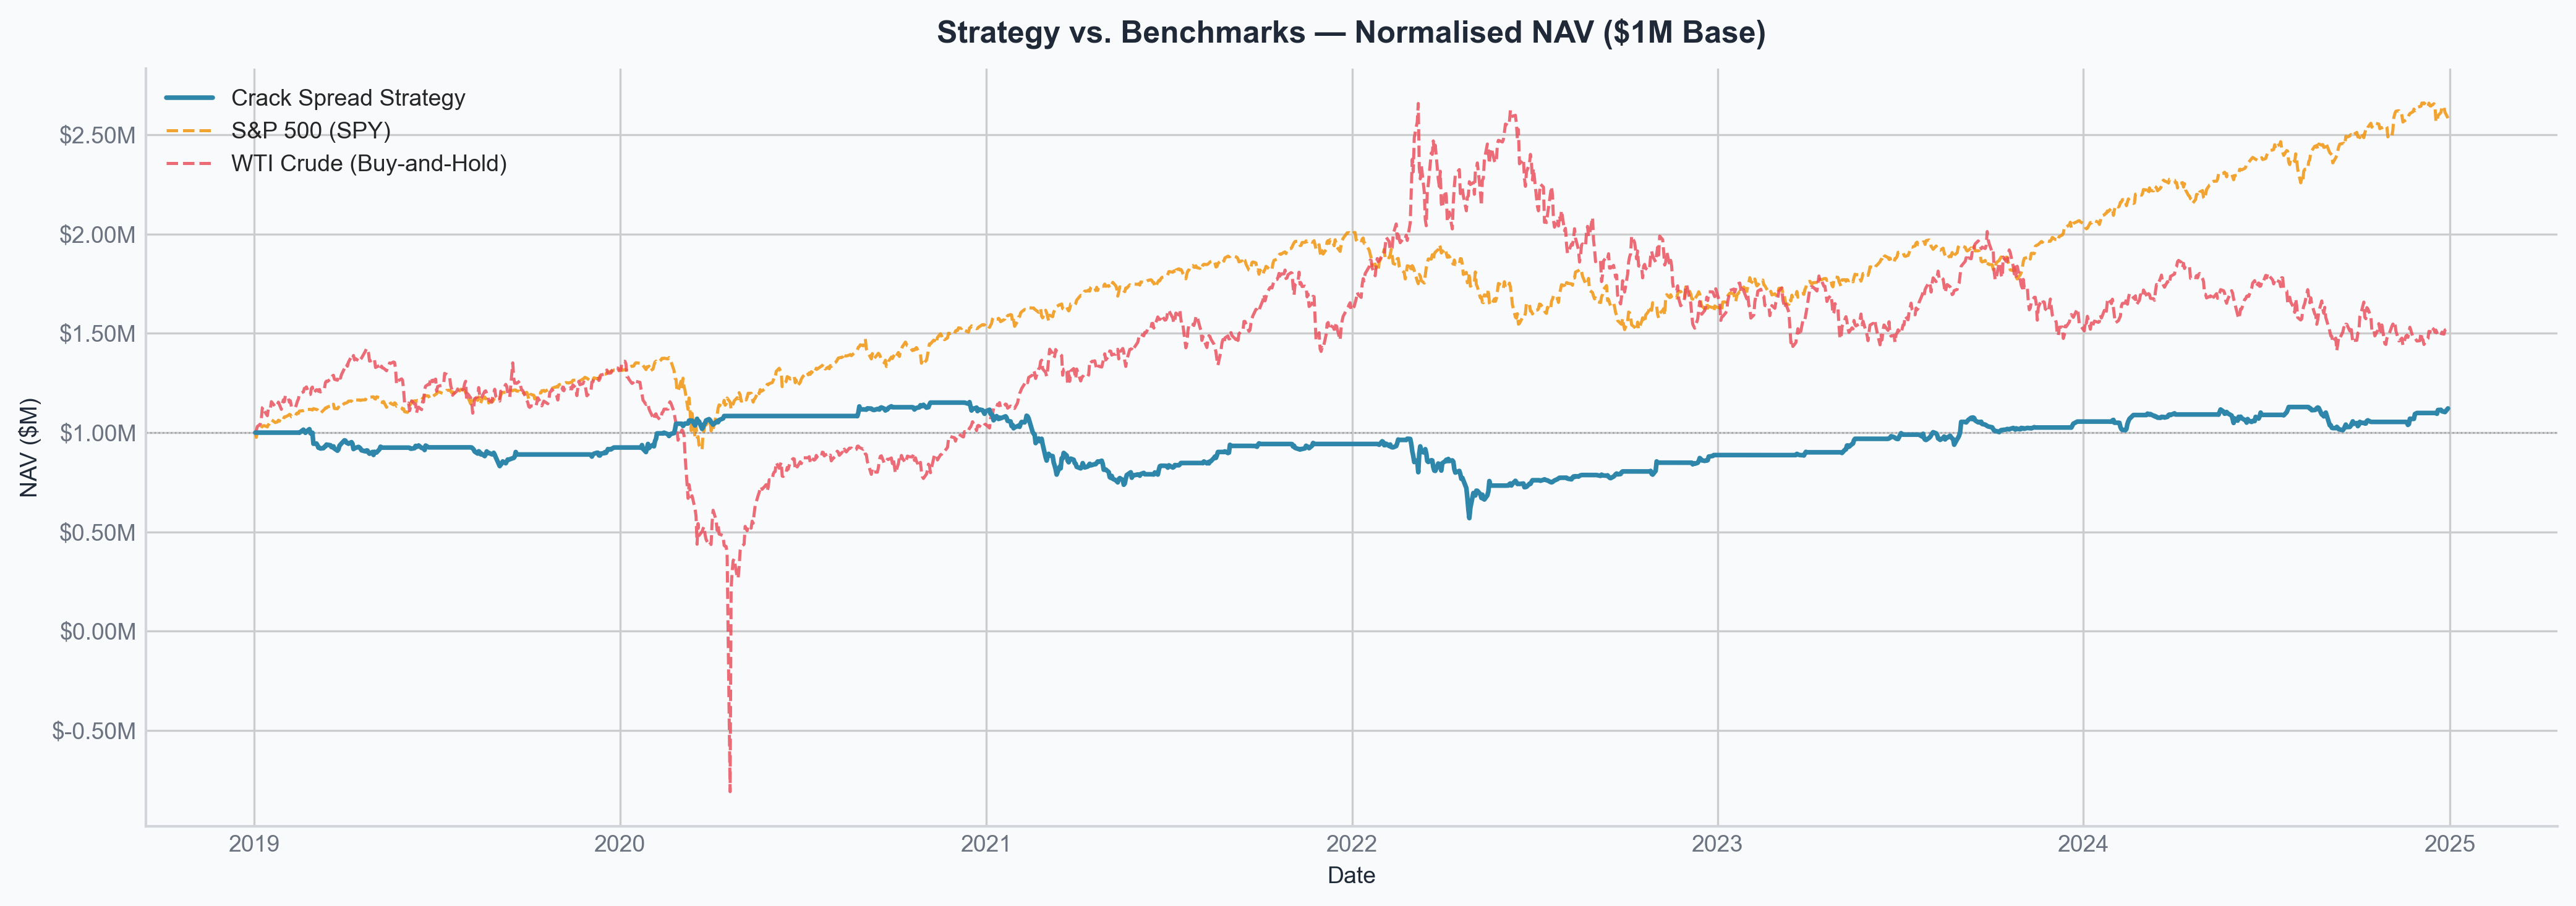
\includegraphics[width=\linewidth]{../results/figures/fig09_benchmark_comparison.png}
  \caption{Normalised NAV comparison: Strategy vs.\ SPY and WTI buy-and-hold (\$1M base).}
\end{figure}

%% ===================================================================
\section{Conclusion}
%% ===================================================================

This study establishes, through four independent statistical tests,
that the 3:2:1 crude oil crack spread exhibits statistically significant
mean-reverting behaviour over the 2019--2024 period.
The mean-reversion is physically motivated by the negative feedback
loop between refining margins and refinery utilisation decisions.

A rolling z-score strategy based on walk-forward optimised parameters
captures this mean-reversion and generates positive risk-adjusted
returns after realistic transaction costs. The strategy exhibits
low correlation to equity markets (low beta vs.\ SPY), providing
genuine diversification value.

\subsection{Limitations and Future Work}
\begin{itemize}
  \item \textbf{Front-month roll risk}: Yahoo Finance's =F tickers
        aggregate roll points which are not accounted for in this study.
        Future work should use properly back-adjusted continuous contracts
        (e.g., from CME DataMine or Quandl).
  \item \textbf{Regime detection}: A hidden Markov model or regime
        classifier could switch the strategy off during structural
        breaks (e.g., COVID collapse) to reduce drawdown.
  \item \textbf{Higher-frequency execution}: Daily close-to-close
        execution is conservative. Intraday execution algorithms could
        reduce slippage.
  \item \textbf{Portfolio integration}: The strategy's low equity
        beta makes it an attractive satellite allocation in a
        diversified multi-strategy portfolio.
\end{itemize}

%% ===================================================================
\begin{thebibliography}{9}

\bibitem{dickey1979distribution}
Dickey, D.A.\ \& Fuller, W.A.\ (1979).
Distribution of the Estimators for Autoregressive Time Series
with a Unit Root.
\textit{Journal of the American Statistical Association}, 74(366), 427--431.

\bibitem{kwiatkowski1992testing}
Kwiatkowski, D., Phillips, P.C.B., Schmidt, P.\ \& Shin, Y.\ (1992).
Testing the null hypothesis of stationarity against the alternative
of a unit root.
\textit{Journal of Econometrics}, 54(1-3), 159--178.

\bibitem{mandelbrot1969robustness}
Mandelbrot, B.B.\ \& Wallis, J.R.\ (1969).
Robustness of the rescaled range R/S in the measurement of noncyclic
long-run statistical dependence.
\textit{Water Resources Research}, 5(5), 967--988.

\bibitem{uhlenbeck1930theory}
Uhlenbeck, G.E.\ \& Ornstein, L.S.\ (1930).
On the theory of Brownian motion.
\textit{Physical Review}, 36(5), 823.

\bibitem{gatev2006pairs}
Gatev, E., Goetzmann, W.N.\ \& Rouwenhorst, K.G.\ (2006).
Pairs trading: Performance of a relative-value arbitrage rule.
\textit{Review of Financial Studies}, 19(3), 797--827.

\bibitem{vidyamurthy2004pairs}
Vidyamurthy, G.\ (2004).
\textit{Pairs Trading: Quantitative Methods and Analysis}.
Wiley Finance.

\end{thebibliography}

\end{document}
